\newpage
\section{It's What the Book Says} 
\begin{teachingnote}
This activity is mostly about careful definitions of these quadrilaterals.  And we want to compare and contrast the two definitions of trapezoid.  
\end{teachingnote}

Fifth graders were given the following task: Put the
terms \textbf{square}, \textbf{rhombus}, and \textbf{parallelogram} in
the Venn diagram below.
\[
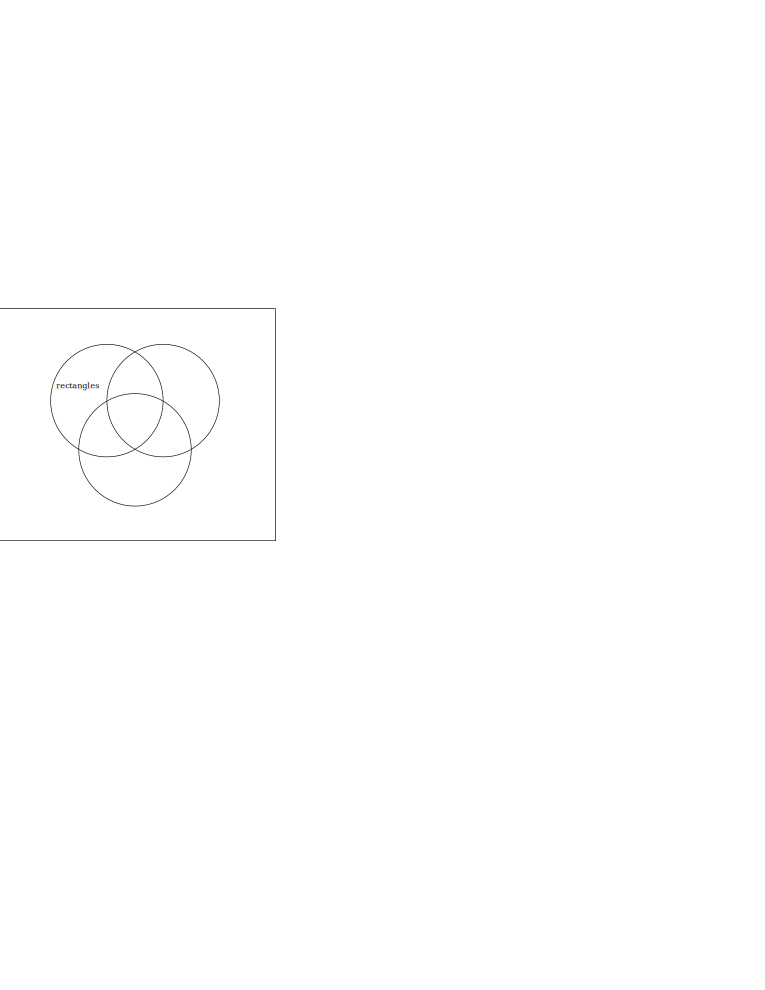
\includegraphics{../graphics/venn.pdf}
\]


\begin{prob} 
What are \textit{squares}, \textit{rhombuses}, and
 \textit{parallelograms}?    
\end{prob}
\vspace{1in}

\begin{prob} 
Critique the question above based on mathematical content.
\end{prob}

\newpage 
\begin{prob}
Supposing we know that a quadrilateral is a polygon with four sides, write clear and succinct definitions of each of the following terms: 
\begin{enumerate}
\itemsep18pt
\item A \textit{rectangle} is a quadrilateral 
\item A \textit{parallelogram} is a quadrilateral
\item A \textit{rhombus} is a quadrilateral
\item A \textit{square} is a quadrilateral
\item A \textit{trapezoid} is a quadrilateral
\item A \textit{kite} is a quadrilateral
\end{enumerate}
\end{prob}
\bigskip

\begin{prob} 
Create a Venn diagram showing the correct relationships
among these quadrilaterals. Be ready to present and defend your
diagram to your peers.
\end{prob}
